\section{Introduction}

\subsection{Balanced \textit{k}-Mean}
	\begin{frame}{Balanced \textit{k}-Means} % FIXME: reorder 3 elements`
		\begin{minipage}{0.5\textwidth} % FIXME: padding
			\textbf{Advantages over classical approaches}
			\begin{itemize}
				\item[$\bullet$] Better targets the global solution of the training problem  
				\item[$\bullet$] Better theoretic scalability on large datasets
			\end{itemize}
		\end{minipage}\hfill
		\begin{minipage}{0.5\textwidth}
			\textbf{Outline}
			\begin{itemize}
				\item[$\bullet$] QUBO formulation and theoretical analysis
				\item[$\bullet$] Empirical Analysis 
				\item[$\bullet$] Conclusions and considerations
			\end{itemize}
		\end{minipage}\hfill
		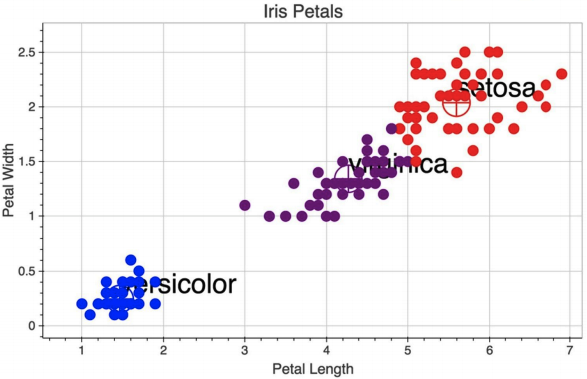
\includegraphics[width=4.3cm]{Iris.png}
	\end{frame}
	% NOTES: We want to cluster data in balanced sets, similarity is 
	% measured by statistical variance withing each cluster
	
	% The advantages ove classical approaches are…
	% This is the outline of the paper of presentation that resembles the one of the paper


\subsection{Unconstrained \textit{k}-Mean Clustering}
	\begin{frame}{Unconstrained \textit{k}-Mean Clustering}
		\textbf{Lloyd’s algorithm}
		\begin{itemize}
			\item[$\bullet$] Complexity $O(Nkdi)$ \textcolor{gray}{[13]}
			\begin{itemize}
				\item[$\circ$] $N$ number of data points
				\item[$\circ$] $k$ number of clusters 
				\item[$\circ$] $d$ dimension of the dataset
				\item[$\circ$] $i$ number of iterations before the algorithm converges
			\end{itemize} 
		\end{itemize}
		\textbf{Scikit-learn implementation}
		\begin{itemize}
			\item[$\bullet$] Complexity $O(Nkd)$ \textcolor{gray}{[18]}
		\end{itemize}
		\tiny{ % FIXME: attach to bottom
			\textcolor{gray}{
				\begin{minipage}{0.5\textwidth} % FIXME: padding
					[13] J. A. Hartigan and M. A. Wong, “Algorithm AS 136: A K-Means clustering algorithm” Applied Statistics
				\end{minipage}\hfill
				\begin{minipage}{0.5\textwidth} 
					[18]“Scikit-learn: Machine learning in python,” J. Mach. Learn. Res.
				\end{minipage}\hfill
			}
		}
	\end{frame}
	

	% Lloyd’s algorithm is an iterative approach for solving unconstrained 
	% k-means clustering (meaning that the result is not necessarily balanced). 
	% The complexity is….

	% The authors use the Scikit-learn implementation (which bounds the number of iterations) as a point of comparison.

\subsection{Balanced \textit{k}-means clustering}
	\begin{frame}{Balanced \textit{k}-means clustering}
		\textbf{Malinen et al.}
		\begin{itemize}
			\item[$\bullet$] Complexity $O(N^3)$ \textcolor{gray}{[13]}
		\end{itemize}
		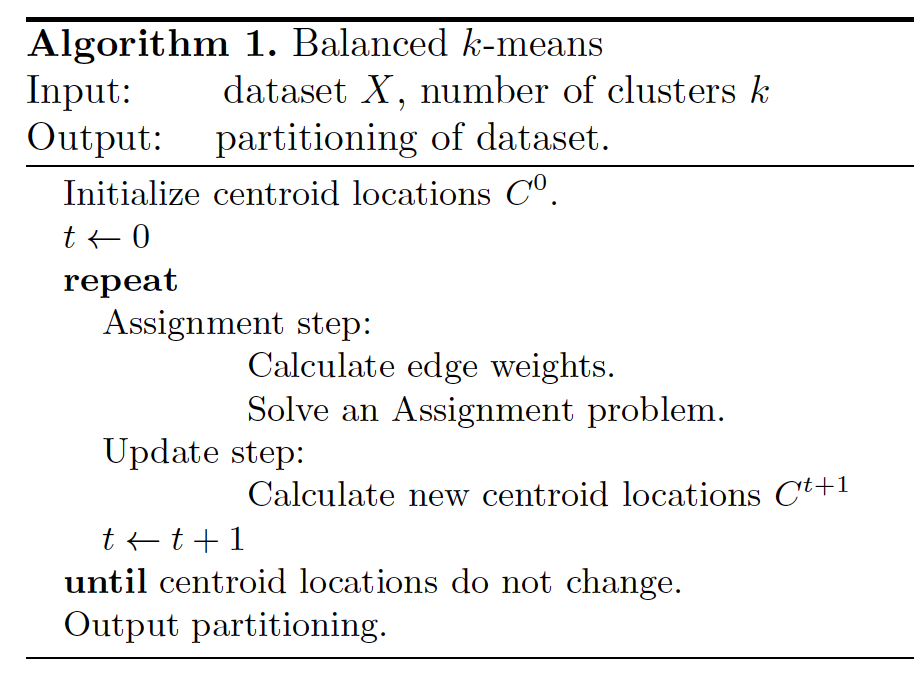
\includegraphics[width=8cm]{[21]algorithm.png}
		\tiny{ % FIXME: attach to bottom
			\textcolor{gray}{
				[21] Malinen, Mikko. (2014). Balanced K-Means for Clustering. 
			}
		}
	\end{frame}

\subsection{Balanced \textit{k}-means clustering}
	\begin{frame}{Balanced \textit{k}-means clustering}
		\begin{columns}
			\begin{column}{0.5\textwidth}
				$$\min _{z \in \mathbb{B}^{M}} z^{T} A z$$

				$$X=\left\{x_{1}, x_{2}, \ldots, x_{N}\right\}$$\\$$\Phi=\left\{\phi_{1}, \phi_{2}, \ldots, \phi_{k}\right\} .$$

				$$\min _{\Phi} \sum_{i=1}^{k} \sum_{x \in \phi_{i}}\left\|x-\mu_{i}\right\|^{2}$$

				$$\min _{\Phi} \sum_{i=1}^{k} \frac{1}{2\left|\phi_{i}\right|} \sum_{x, y \in \phi_{i}}\|x-y\|^{2}$$

			\end{column}
			\begin{column}{0.5\textwidth}  
				$$\min _{\Phi} \sum_{i=1}^{k} \sum_{x, y \in \phi_{i}}\|x-y\|^{2}$$

				Distance matrix: $D$ \\Assignment matrix: $\hat W$

				$$\sum_{x, y \in \phi_{j}}\|x-y\|^{2}=\hat{w}_{j}^{T} D \hat{w}_{j}^{\prime}$$

				$$\min _{\hat{w}} \hat{w}^{T}\left(I_{k} \otimes D\right) \hat{w}$$

			\end{column}
		\end{columns}
	\end{frame}
	% 	Quantum clustering algorithms have been proposed, however, none target the exact solution to the k-means or balanced k-means clustering model. Instead, they are heuristic approaches that approximate the k-means optimization problem. We propose a QUBO formulation that is identical to the balanced k-means training problem. 
	% Our goal is to convert the balanced k-means training problem into a QUBO formulation. 
	% 1-> A is the real valued MxM QUBO matrix while z is the binary decision vector
	% 2-> we want to partition a dataset of N samples into k clusters
	% 3-> mu is the centroid of a cluster
	% 4-> utilizing the law of total variance
	% 5-> in case we assume the clusters to be
	% 6-> NxN matrix with distances, Nxk matrix with binary values with ones if a sample is assigned to that column's cluster
	% 7-> w_j is the j-th column of W the first multiplication makes us obtain a n-row vector in which each value is the sum of the distances of 1 of n samples from the samples in the cluster, the second one only select the sum of distances of samples in the same cluster.
	% 8-> \hat w is the vertical stack of column of W, now need to add the constraint over \hat W through penalties 



\section{QUBO Formulation}